\chapter{Latex}
LaTeX is a document preparation system for high-quality typesetting. It is most often used for medium-to-large technical or scientific documents but it can be used for almost any form of publishing. 

\marginnote
\begin{figure}	
    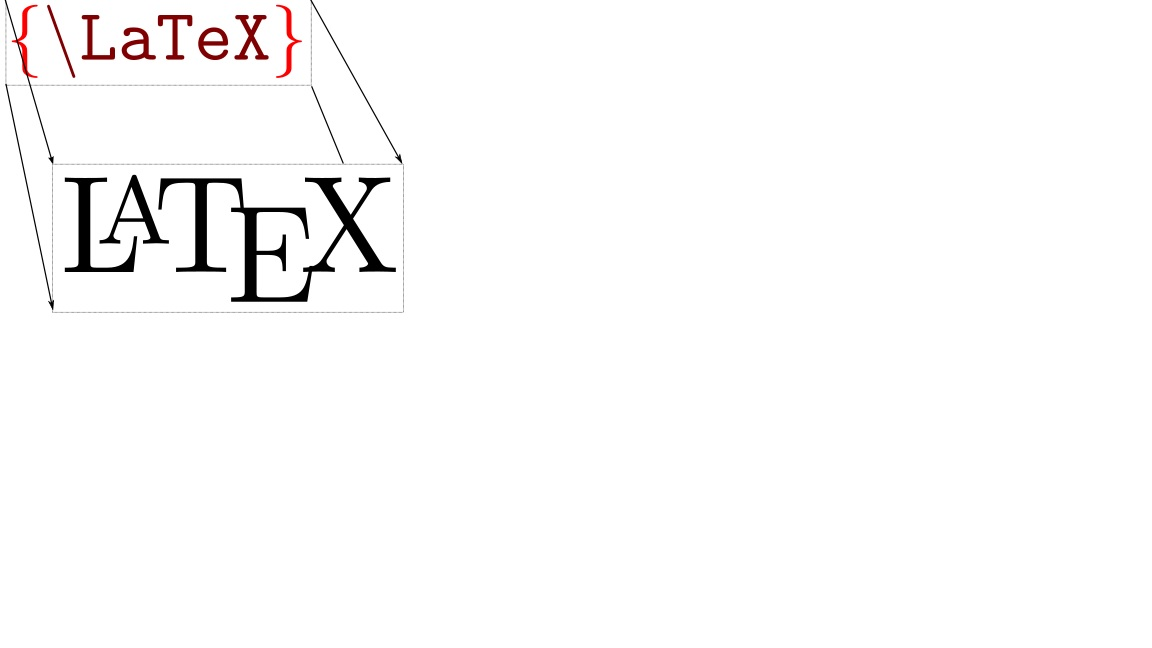
\includegraphics[width=10cm]{1}
\end{figure}

\section{Using of the latex}

The Latex is used for writing the essay such as about Codes, mathmatic functions, graphics etc. This tool is useful as you try to put images into your assignment, because there are a lot of ways to do it. Actually not only putting images but also differentiating the section of your part. 

\begin{figure}
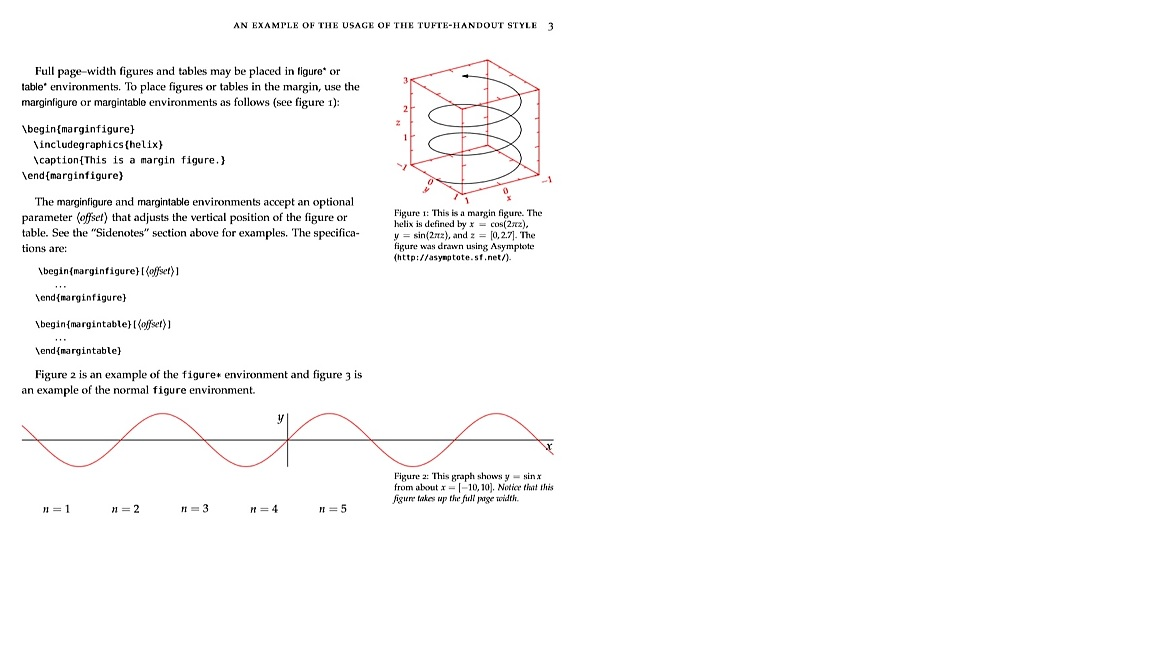
\includegraphics[width=10cm]{123}
\end{figure}

\section{The features of using Latex}
A.Typesetting journal articles, technical reports, books, and slide presentations.
B.Control over large documents containing sectioning, cross-references, tables and figures.
C.Typesetting of complex mathematical formulas.
D.Advanced typesetting of mathematics with AMS-LaTeX.
E.Automatic generation of bibliographies and indexes.
F.Multi-lingual typesetting.
G.Inclusion of artwork, and process or spot colour.
H.Using PostScript or Metafont fonts.

\begin{figure}
	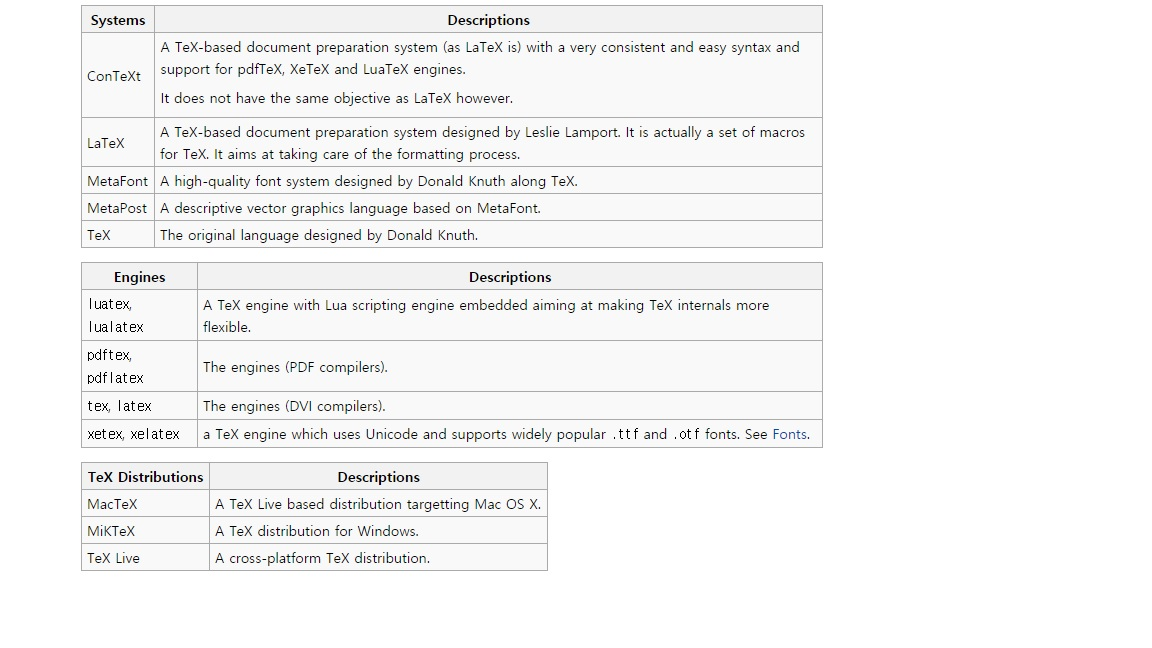
\includegraphics[width=10cm]{234}
\end{figure}

Latex is also easy to use for beginner There are a lot of tools to begin writing essaies. When beginner doesn't know how to use, they would be able to search the solutions from the internet web sites. 
